\begin{singlespace}
    \chapter{\textbf{Appendix C: \\ Supplemental material for "The relative cost of resource use for photosynthesis drives variance in leaf nitrogen content across a climate and soil resource availability gradient"}}
\end{singlespace}

\setcounter{table}{0}
\renewcommand{\thetable}{C\arabic{table}}

\setcounter{table}{0}
\renewcommand{\thefigure}{C\arabic{figure}}


\section*{C.1 Calculations for soil water holding capacity}

Water holding capacity ($\theta_\mathrm{WHC}$; mm) was calculated as a function of the volumetric soil water storage at field capacity ($W_\mathrm{FC}$; $\mathrm{m^3\ m^{-3}}$), and the volumetric soil water storage at wilting point ($W_\mathrm{PWP}$; $\mathrm{m^3\ m^{-3}}$):

\begin{equation}
    \label{eqn_s4.1} \tag{C4.1}
    \theta_{WHC} = (W_{FC}-W_{PWP})(1-f_{gravel}) * min(z_{bedrock}, z_{max})
\end{equation}

\noindent where $f_\mathrm{gravel}$ (\%) is the fraction of gravel content in soil, $z_\mathrm{bedrock}$ (mm) is the distance to bedrock, and $z_\mathrm{max}$ (mm) is the maximum allowable distance to bedrock, set to 2000mm. $W_\mathrm{FC}$ is calculated as:

\begin{equation}
    \label{eqn_s4.2} \tag{C4.2}
    \theta_{FC} = k_{fc}+(1.283*(k_{fc})^2-0.374*k_{fc}-0.015)
\end{equation}

\noindent where

\begin{equation}
    \label{eqn_s4.3} \tag{C4.3}
    \begin{aligned}
        k_{fc}= -0.251 * f_{sand} + 0.195 * f_{clay} + 0.011 * f_{OM} \\ + 0.006 * (f_{sand} * f_{OM}) - 0.027 * (f_{clay} \\ * f_{OM}) + 0.452 * (f_{sand} * f_{clay}) + 0.299
    \end{aligned}	
\end{equation}

\noindent $W_\mathrm{PWP}$ is calculated as:

\begin{equation}
    \label{eqn_s4.4} \tag{C4.4}
    W_{PWP}=k_{pwp}+(0.14*k_{pwp}-0.02)	
\end{equation}

\noindent where

\begin{equation}
    \label{eqn_s4.5} \tag{C4.5}
    \begin{aligned}
        k_{pwp} = -0.024 * f_{sand} + 0.487 * f_{clay} + 0.006 * f_{OM} \\ + 0.005 * (f_{sand} * f_{OM}) - 0.013 * (f_{clay} \\ * f_{OM}) + 0.068 * (f_{sand} * f_{clay}) + 0.031
    \end{aligned}
\end{equation}

\noindent In Equations \ref{eqn_s4.4} and \ref{eqn_s4.5}, $f_\mathrm{sand}$ (\%) is the fraction of sand content in soil (\%), $f_\mathrm{clay}$ (\%) is the fraction of clay content in soil (\%), and $f_\mathrm{OM}$ is the fraction of organic matter in soil (\%). Organic matter in the soil was calculated in this study by converting soil organic carbon data extracted from SoilGrids 2.0 to soil organic matter using the van Bemmelen factor (1.724 conversion factor).
\clearpage


\begin{landscape}
    \begin{table}[]
        \caption{List of sampled species and their plant functional group assignment}
        \resizebox{\columnwidth}{!}{%
            \begin{tabular}{p{2cm}p{5cm}p{2cm}p{2cm}p{2cm}p{2cm}p{3.5cm}p{2cm}}
            \hline
            \textbf{Symbol} & \textbf{Species} & \textbf{\begin{tabular}[c]{@{}l@{}}Photo.\\ pathway\end{tabular}} &
            \textbf{\begin{tabular}[c]{@{}l@{}}Growth\\ duration\end{tabular}} & \textbf{Growth  habit} &
            \textbf{N-fixer?} & \textbf{\begin{tabular}[c]{@{}l@{}}Plant functional \\ group\end{tabular}} &
            \multicolumn{1}{l}{\textbf{\begin{tabular}[c]{@{}l@{}}Number \\ sampled\end{tabular}}} \\
            \hline
            ACAN11 & \textit{Acaciella angustissima}    & c3 & perennial & forb           & yes & c3\_legume    & 3  \\
            AMAR2  & \textit{Ambrosia artemisiifolia}   & c3 & annual    & forb           & no  & c3\_nonlegume & 25 \\
            AMPS   & \textit{Ambrosia psilostachya}     & c3 & perennial & forb           & no  & c3\_nonlegume & 32 \\
            ARAL3  & \textit{Argemone albiflora}        & c3 & annual    & forb           & no  & c3\_nonlegume & 3  \\
            ARPU9  & \textit{Aristida purpurea}         & c4 & perennial & graminoid      & no  & c4\_nonlegume & 2  \\
            ASAS   & \textit{Asclepias asperula}        & c3 & perennial & forb           & no  & c3\_nonlegume & 3  \\
            ASLA4  & \textit{Asclepias latifolia}       & c3 & perennial & forb           & no  & c3\_nonlegume & 3  \\
            ASSY   & \textit{Asclepias syriaca}         & c3 & perennial & forb           & no  & c3\_nonlegume & 18 \\
            BASA   & \textit{Baccharis salicina}        & c3 & perennial & shrub          & no  & c3\_nonlegume & 3  \\
            BOIS   & \textit{Bothriochloa ischaemum}    & c4 & perennial & graminoid      & no  & c4\_nonlegume & 6  \\
            BOSA   & \textit{Bothriochloa saccharoides} & c4 & perennial & graminoid      & no  & c4\_nonlegume & 6  \\
            CAAM2  & \textit{Callicarpa americana}      & c3 & perennial & shrub          & no  & c3\_nonlegume & 3  \\
            CAPL3  & \textit{Carex planostachys}        & c4 & perennial & graminoid      & no  & c4\_nonlegume & 3  \\
            CAREX  & Carex spp.                         & c4 & perennial & graminoid      & no  & c4\_nonlegume & 16 \\
            CHFE3  & \textit{Chamaesyce fendleri}       & c3 & perennial & forb           & no  & c3\_nonlegume & 2  \\
            CHPI8  & \textit{Chyrysopsis pilosa}        & c3 & annual    & forb           & no  & c3\_nonlegume & 3  \\
            COCO13 & \textit{Conoclinium coelestinum}   & c3 & perennial & forb           & no  & c3\_nonlegume & 3  \\
            COER   & \textit{Commelina erecta}          & c3 & perennial & forb           & no  & c3\_nonlegume & 3  \\
            CRGLL  & \textit{Croton glandulosus}        & c3 & annual    & forb           & no  & c3\_nonlegume & 22 \\
            CYDA   & \textit{Cynodon dactylon}          & c4 & perennial & graminoid      & no  & c4\_nonlegume & 15 \\
            DATE3  & \textit{Dasylirion texanum}        & c3 & perennial & shrub          & no  & c3\_nonlegume & 3  \\
            DIAN   & \textit{Dichanthium annulatum}     & c4 & perennial & graminoid      & no  & c4\_nonlegume & 8  \\
            ENPE4  & \textit{Engelmannia peristenia}    & c3 & perennial & forb           & no  & c3\_nonlegume & 6  \\
            EUMA8  & \textit{Euphorbia marginata}       & c3 & annual    & forb           & no  & c3\_nonlegume & 6  \\
            GAPU   & \textit{Gaillardia pulchella}      & c3 & annual    & forb           & no  & c3\_nonlegume & 16 \\
            GLGO   & \textit{Glandularia gooddingii}    & c3 & perennial & forb           & no  & c3\_nonlegume & 2  \\
            HEAN3  & \textit{Helianthus annuus}         & c3 & annual    & forb           & no  & c3\_nonlegume & 6  \\
        \end{tabular}}
    \end{table}
\end{landscape}
\clearpage

\newpage
\begin{landscape}
    \begin{table}[]
        \caption{List of sampled species and their plant functional group assignment (cont.)}
        \resizebox{\columnwidth}{!}{%
            \begin{tabular}{p{2cm}p{5cm}p{2cm}p{2cm}p{2cm}p{2cm}p{3.5cm}p{2cm}}
        \hline
        \textbf{Symbol} & \textbf{Species} & \textbf{\begin{tabular}[c]{@{}l@{}}Photo.\\ pathway\end{tabular}} &
        \textbf{\begin{tabular}[c]{@{}l@{}}Growth\\ duration\end{tabular}} & \textbf{Growth habit} &
        \textbf{N-fixer?} & \textbf{\begin{tabular}[c]{@{}l@{}}Plant functional \\ group\end{tabular}} &
        \multicolumn{1}{l}{\textbf{\begin{tabular}[c]{@{}l@{}}Number \\ sampled\end{tabular}}} \\
        \hline
        HECA8  & \textit{Heterotheca canescens}     & c3 & perennial & forb           & no  & c3\_nonlegume & 2  \\
        HETE3  & \textit{Heliotropium tenellum}     & c3 & annual    & forb           & no  & c3\_nonlegume & 3  \\
        IVAX   & \textit{Iva axillaris}             & c3 & perennial & forb           & no  & c3\_nonlegume & 4  \\
        LIAT   & \textit{Lilaeopsis attenuata}      & c3 & perennial & forb           & no  & c3\_nonlegume & 3  \\
        LIPU   & \textit{Liatris punctata}          & c3 & perennial & forb           & no  & c3\_nonlegume & 3  \\
        LOPE   & \textit{Lolium perenne}            & c3 & perennial & graminoid      & no  & c3\_nonlegume & 9  \\
        MIQU2  & \textit{Mimosa quadrivalvis}       & c3 & perennial & forb           & yes & c3\_legume    & 15 \\
        NALE3  & \textit{Nassella leucotricha}      & c3 & perennial & graminoid      & no  & c3\_nonlegume & 19 \\
        OECU2  & \textit{Oenothera curtiflora}      & c3 & annual    & forb           & no  & c3\_nonlegume & 3  \\
        OENOT  & Oenothera spp.                     & c3 & annual    & forb           & no  & c3\_nonlegume & 1  \\
        PAVI2  & \textit{Panicum virgatum}          & c4 & perennial & graminoid      & no  & c4\_nonlegume & 12 \\
        PRGL2  & \textit{Prosopis glandulosa}       & c3 & perennial & shrub          & yes & c3\_legume    & 33 \\
        QUHA3  & \textit{Quercus harvardii}         & c3 & perennial & shrub          & no  & c3\_nonlegume & 3  \\
        QUMO   & \textit{Quercus mohriana}          & c3 & perennial & shrub          & no  & c3\_nonlegume & 1  \\
        RACO3  & \textit{Ratibida columnifera}      & c3 & perennial & forb           & no  & c3\_nonlegume & 40 \\
        RHAM   & Rhamnus spp.                       & c3 & perennial & shrub          & yes & c3\_legume    & 1  \\
        RHSET  & \textit{Rhynchosia senna}          & c3 & perennial & forb           & yes & c3\_legume    & 1  \\
        RUHI2  & \textit{Rudbeckia hirta}           & c3 & perennial & forb           & no  & c3\_nonlegume & 3  \\
        RUNU   & \textit{Ruellia nudiflora}         & c3 & perennial & forb           & no  & c3\_nonlegume & 15 \\
        RUTR   & \textit{Rubus trivialis}           & c3 & perennial & vine           & no  & c3\_nonlegume & 3  \\
        SAFA2  & \textit{Salvia farinacea}          & c3 & perennial & forb           & no  & c3\_nonlegume & 7  \\
        SCHIZ4 & Schizachyrium spp.                 & c4 & perennial & graminoid      & no  & c4\_nonlegume & 8  \\
        SCSC   & \textit{Schizachyrium scoparium}   & c4 & perennial & graminoid      & no  & c4\_nonlegume & 3  \\
        SODI   & \textit{Solanum dimidiatum}        & c3 & perennial & forb           & no  & c3\_nonlegume & 1  \\
        SOEL   & \textit{Solanum elaeagnifolium}    & c3 & perennial & forb           & no  & c3\_nonlegume & 53 \\
        SOHA   & \textit{Sorghum halapense}         & c4 & perennial & graminoid      & no  & c4\_nonlegume & 38 \\
        STTE3  & \textit{Stillingia texana}         & c3 & perennial & forb           & no  & c3\_nonlegume & 3
    \end{tabular}}
\end{table}
\end{landscape}
\clearpage

\newpage
\begin{landscape}
    \begin{table}
        \caption{List of sampled species and their plant functional group assignment (cont.)}
        \resizebox{\columnwidth}{!}{%
            \begin{tabular}{p{2cm}p{5cm}p{2cm}p{2cm}p{2cm}p{2cm}p{3.5cm}p{2cm}}
            \hline
            \textbf{Symbol} & \textbf{Species} & \textbf{\begin{tabular}[c]{@{}l@{}}Photo.\\ pathway\end{tabular}} &
            \textbf{\begin{tabular}[c]{@{}l@{}}Growth\\ duration\end{tabular}} & \textbf{Growth habit} &
            \textbf{N-fixer?} & \textbf{\begin{tabular}[c]{@{}l@{}}Plant functional \\ group\end{tabular}} &
            \multicolumn{1}{l}{\textbf{\begin{tabular}[c]{@{}l@{}}Number \\ sampled\end{tabular}}} \\
            \hline
            VEOC   & \textit{Verbesina occidentalis}    & c3 & perennial & forb           & no  & c3\_nonlegume & 3  \\
            VEST   & \textit{Verbena stricta}           & c3 & perennial & forb           & no  & c3\_nonlegume & 3  \\
            WEAC   & \textit{Wedelia acapulcensis}      & c3 & perennial & shrub          & no  & c3\_nonlegume & 6 
        \end{tabular}}
    \end{table}
\end{landscape}
\clearpage


\newpage
\begin{table}[]
    \caption{Model selection results for soil moisture, air temperature, and vapor pressure deficit. Soil moisture was used in a bivariate regression against $\beta$, while vapor pressure deficit was used in bivariate regressions against leaf $C_\mathrm{i}$:$C_\mathrm{a}{}^*$}
    \resizebox{\columnwidth}{!}{%
        \begin{tabular}{p{2cm}p{2cm}p{2cm}p{2cm}p{2cm}}
            & \multicolumn{2}{l}{Soil moisture} & \multicolumn{2}{l}{VPD} \\
            \hline
            Day & AICc             & RMSE           & AICc        & RMSE      \\
            \hline
            1   & 1431.77          & 0.8400         & -772.71           & 0.0853    \\
            2   & 1431.76          & 0.8400         & -775.47           & 0.0849    \\
            3   & 1431.78          & 0.8400         & -770.86           & 0.0854    \\
            4   & 1431.79          & 0.8401         & \textbf{-793.49}  & \textbf{0.0839}    \\
            5   & 1431.79          & 0.8401         & -771.66           & 0.0853    \\
            6   & 1431.78          & 0.8401         & -771.66           & 0.0853    \\
            7   & 1431.78          & 0.8401         & -771.05           & 0.0854    \\
            8   & 1431.76          & 0.8401         & -770.94           & 0.0854    \\
            9   & 1431.75          & 0.8401         & -770.11           & 0.0854    \\
            10  & 1431.74          & 0.8401         & -770.08           & 0.0855    \\
            15  & 1431.54          & 0.8401         & -768.64           & 0.0856    \\
            20  & 1431.40          & 0.8401         & -769.77           & 0.0855    \\
            30  & 1431.23          & 0.8400         & -772.18           & 0.0853    \\
            60  & 1429.84          & 0.8391         & -779.06           & 0.0848    \\
            90  & \textbf{1429.14} & \textbf{0.8385}& -773.99           & 0.0852    
\end{tabular}%
}
\end{table}
\clearpage

\newpage
\begin{landscape}
    \begin{figure}
        \centering
        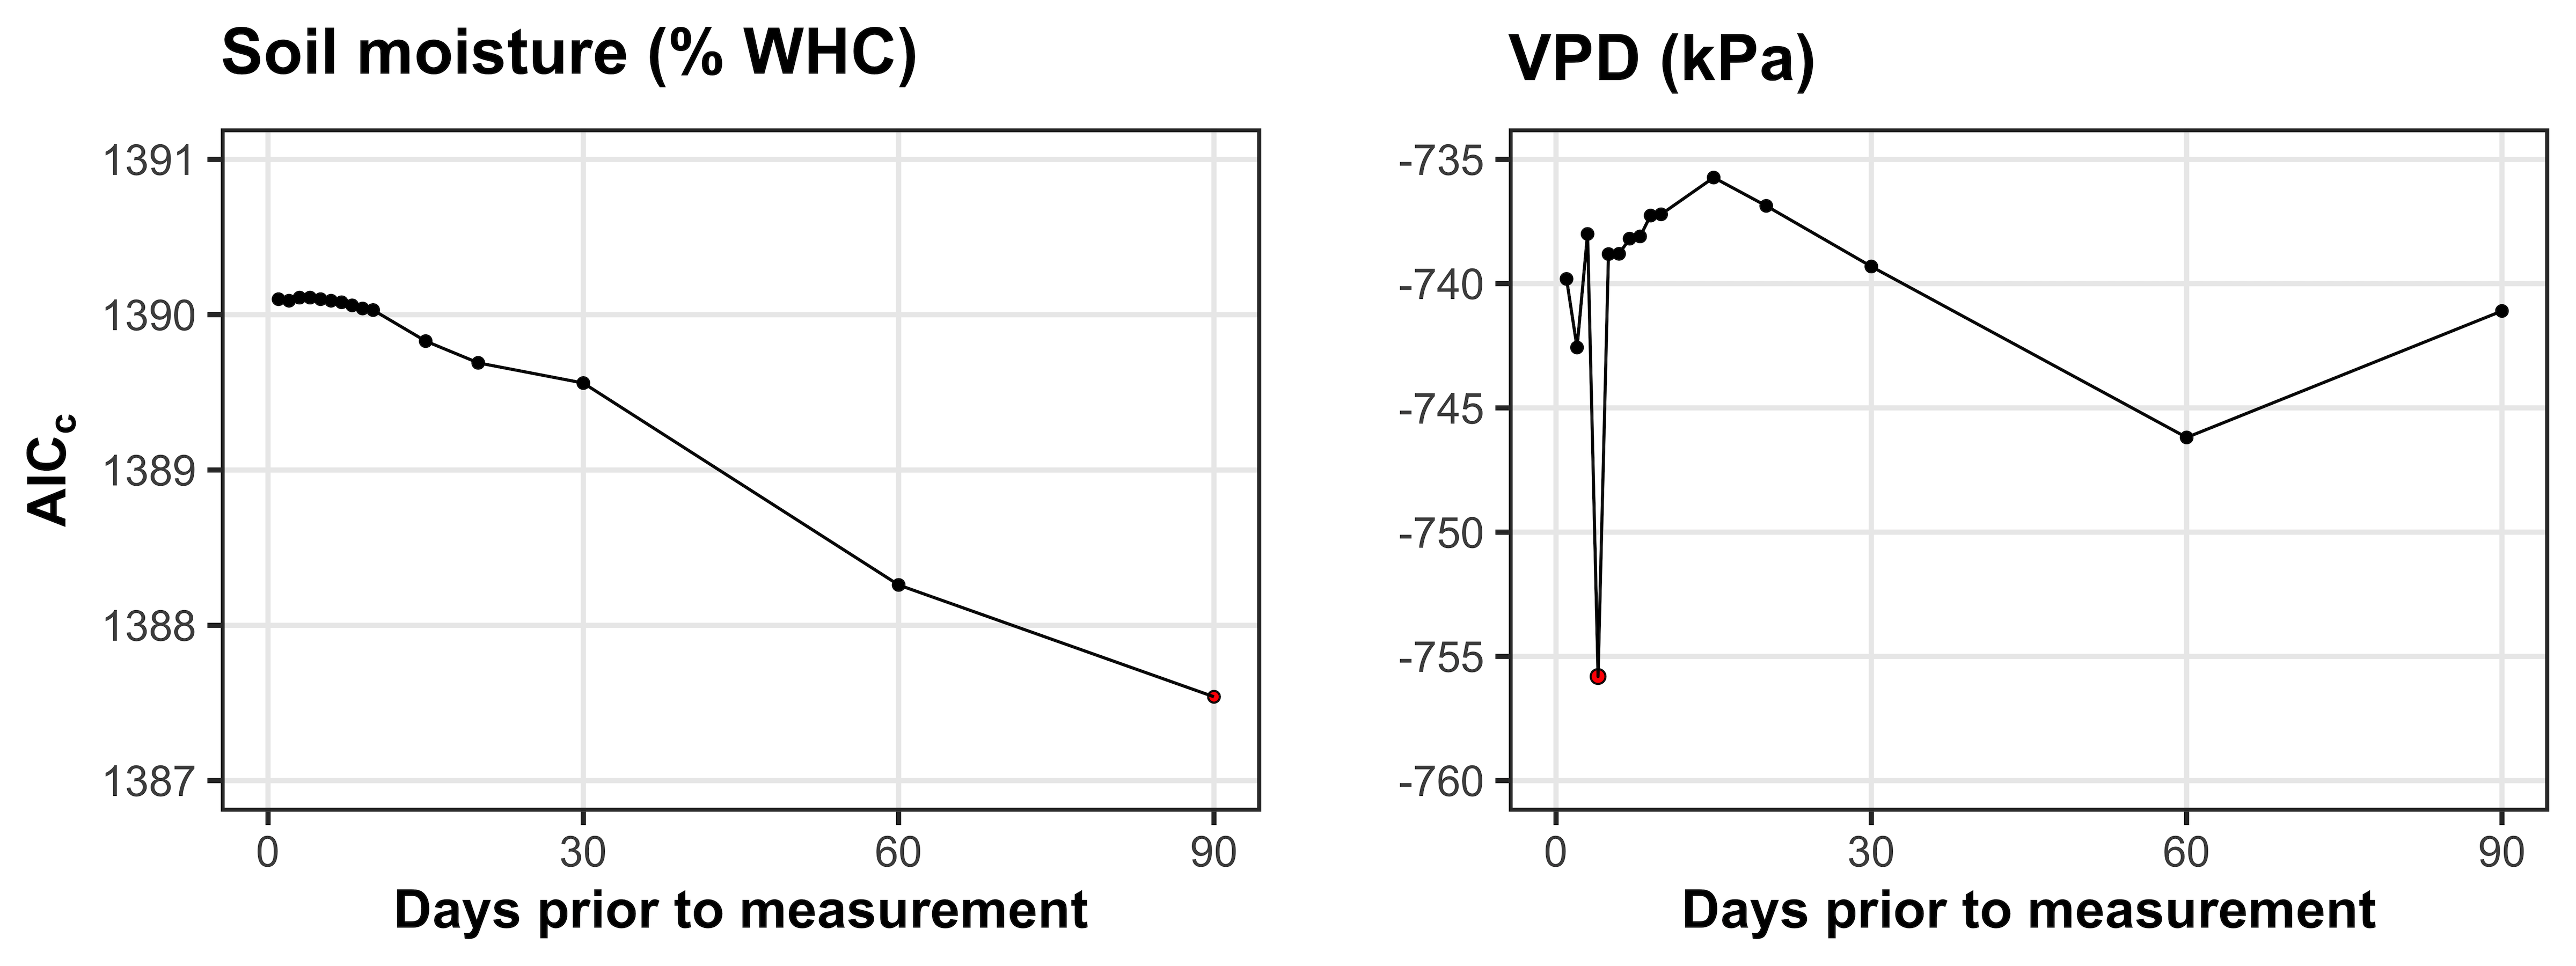
\includegraphics[scale = 0.07]{ch4_TXeco/figs/TXeco_figS2_aicc.png}
        \caption[Model selection results exploring relevant timescales for soil moisture and vapor pressure deficit]{Model selection results exploring relevant timescales for soil moisture (left panel) and vapor pressure deficit (right panel). The x-axis indicates the number of days before each site visit and the y-axis notes the corrected Akaike Information Criterion value. The timescale with the lowest AICc value, and therefore most relevant timescale to include in statistical models, is noted as a red point.}
        \label{fig:figurec.1}
    \end{figure}
\end{landscape}
\clearpage

